%-------------------------------
%	DOCUMENT SETTINGS
%-------------------------------
\documentclass[a4paper]{article}

\setlength{\hoffset}{-3.2cm}
\setlength{\voffset}{-3cm}
\setlength{\textwidth}{18.7cm}
\setlength{\textheight}{25.5cm}
\setlength{\parskip}{0pt}
\setlength{\parindent}{0in}

%----------------------------------------------------------------------------------------
%	PACKAGES AND OTHER DOCUMENT CONFIGURATIONS
%----------------------------------------------------------------------------------------

\usepackage{minted}
\usepackage{mathtools}
\usepackage[utf8]{inputenc} % Use UTF-8 encoding
\usepackage{microtype} % Slightly tweak font spacing for aesthetics
\usepackage[english]{babel} % Language hyphenation and typographical rules
\usepackage{amsthm, amsmath, amssymb} % Mathematical typesetting
\usepackage{float} % Improved interface for floating objects
\usepackage[final, colorlinks = true, linkcolor = black, citecolor = black]{hyperref} % For hyperlinks in the PDF
\usepackage{dsfont}
\DeclarePairedDelimiter\abs{\lvert}{\rvert}%
\usepackage{cancel}
\usepackage{charter} % Use the Charter font
\usepackage{graphicx, multicol} % Enhanced support for graphics
\usepackage{xcolor} % Driver-independent color extensions
\usepackage{booktabs} % Enhances quality of tables
\usepackage{tikz-qtree} % Easy tree drawing tool
% Configuration for b-trees and b+-trees, !uses style file!
%\usepackage[backend=biber,style=numeric,
%            sorting=nyt]{biblatex} % Complete reimplementation of bibliographic facilities
%\addbibresource{ecl.bib}
\usepackage[yyyymmdd]{datetime} % Uses YEAR-MONTH-DAY format for dates
\renewcommand{\dateseparator}{-} % Sets dateseparator to '-'
\usepackage{fancyhdr} % Headers and footers
\pagestyle{fancy} % All pages have headers and footers
\fancyhead{}\renewcommand{\headrulewidth}{0pt} % Blank out the default header
\fancyfoot[L]{} % Custom footer text
\fancyfoot[C]{} % Custom footer text
\fancyfoot[R]{\thepage} % Custom footer text
\newcommand{\note}[1]{\marginpar{\scriptsize \textcolor{red}{#1}}} % Enables comments in red on margin

%----------------------------------------------------------------------------------------
%	CUSTOM COMMANDS
%----------------------------------------------------------------------------------------

\newcommand{\R}{\mathbb{R}}
\newcommand{\E}{\mathbb{E}}
\newcommand{\I}{\mathbb{I}}
\newcommand{\Var}{\text{Var}}
% Para poner sonrisa sobre puntos suspensivos. Uso: \overplace{n}{\dotsc}
\newcommand{\overplace}[2]{%
	\overset{\substack{#1\\\smile}}{#2}%
}

\begin{document}
	
%-------------------------------
%	TITLE SECTION
%-------------------------------

\fancyhead[C]{}
\hrule \medskip % Upper rule
\begin{minipage}{0.295\textwidth} 
	\raggedright
	\footnotesize
	José Antonio Álvarez Ocete \hfill\\   
	77553417Q \hfill\\
	joseantonio.alvarezo@estudiante.uam.es
\end{minipage}
\begin{minipage}{0.4\textwidth} 
	\centering 
	\large 
	Final \\ 
	\normalsize 
	Procesos estocásticos discretos\\ 
\end{minipage}
\begin{minipage}{0.295\textwidth} 
	\raggedleft
	\today\hfill\\
\end{minipage}
\medskip\hrule 
\bigskip

%-------------------------------
%	CONTENTS
%-------------------------------

\section*{Ejercicio I.}

\textbf{Enunciado.} En los apuntes hay el ejemplo del \emph{gambler's ruin} como cadena de Markov:

\begin{figure}[H]
	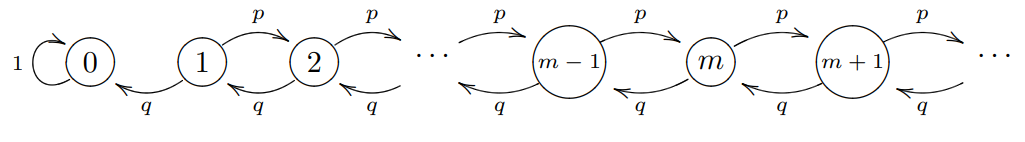
\includegraphics[scale=.6]{figures/gamblers_ruin}
	\centering
\end{figure}

Donde estar en el nodo $i$ implica tener $i$ Euros, y $p$ y $q=1-p$ son las probabilidades de ganar y perder respectivamente en cada repetición del juego. \\

\textbf{Apartado a)} Hacer un gráfico del número medio de jugadas que el jugador puede hacer antes de arruinarse en función del dinero inicial. En cada jugada se juega $1$ Euro, y el juego es ecuo (el jugador tiene una probabilidad $p=1/2$ de ganar). \\

Sabemos por el estudio teórico realizado para este problema que en el caso de $p=q=\frac{1}{2}$, el jugador convergerá a arruinarse tarde o temprano. Sin embargo, la simulación puede tomar un tiempo arbitrariamente alto de tiempo si el dinero inicial es alto. Es por ello que hemos de poner un límite al número de iteraciones máximo que ejecutaremos nuestra simulación. Consideramos que $10^5$ es una cantidad aceptable de iteraciones para los bajos valores de dinero inicial que utilizaremos. Si se alcanza ese número de iteraciones podemos considerar que el jugador "se arruina en tiempo $10^5$, que es básicamente infinito. \\

Implementamos la simulación de esta cadena de Markov y la ejecutamos $20$ veces, computando su media. Realizar esta simulación en múltiples ocasiones y utilizar la media es imprescindible para obtener resultados representativos en procesos de Monte Carlo como este. Cabe destacar que para cualquiera de estos experimentos fijamos la semilla a $123$ para poder reproducirlos posteriormente.
	
\begin{minted}{python}
def simulate_gambler_step(p=1/2):
	""" 
		Simulates a single step of the gambler's ruin
		- p: the probability of winning
		- returns: 1 if won, -1 if lost
	"""
	r = random.uniform(0, 1)
	return 1 if r <= p else -1

def simulate_gamblers_ruin(initial_money, p=1/2, max_steps=10**6):
	"""
		Simulates a gambler's ruin markov chain.
		- initial_money: the starting node
		- p: the probability of winning at each step
		- max_steps: the max number of steps to be comptued
		- returns: time taken to ruin the gambler. If max_steps is reached
		without ruining the gambler, return max_steps instead.
	"""
	money = initial_money
	steps = 0
	while money > 0 and steps <= max_steps:
	steps += 1
	money += simulate_gambler_step(p)
	return steps

def plot_mean_ruin_time(max_initial_money=50, n=20, max_steps=10**5, p=1/2):
	"""
		Plots the mean time for a gambler's to ruin themself, against the initial money.
		- max_initial_money: max initial money to be plotted
		- n: the number of executions per initial money value
		- max_steps: the max number of steps to be comptued
		- p: the probability of winning at each step
	"""
	# Compute times
	initial_money_range = np.arange(1, max_initial_money)
	mean_times = [
		np.mean( [simulate_gamblers_ruin(initial_money, p=p, max_steps=max_steps)
				for _ in range(n)] )
		for initial_money in initial_money_range
	]

	# Plotting
	plt.figure(figsize=(12,6))
	plt.plot(initial_money_range, mean_times, '-o')
	plt.legend(['Mean time to ruin', 'Max iterations'])
	plt.xlabel('Initial money')
	plt.ylabel('Mean time to ruin in {} iterations'.format(n))
	plt.title('Gambler\' ruin simulation')
	plt.show()
	
random.seed(123)
plot_mean_ruin_time(max_steps=10**5)
\end{minted}
	
\begin{figure}[H]
	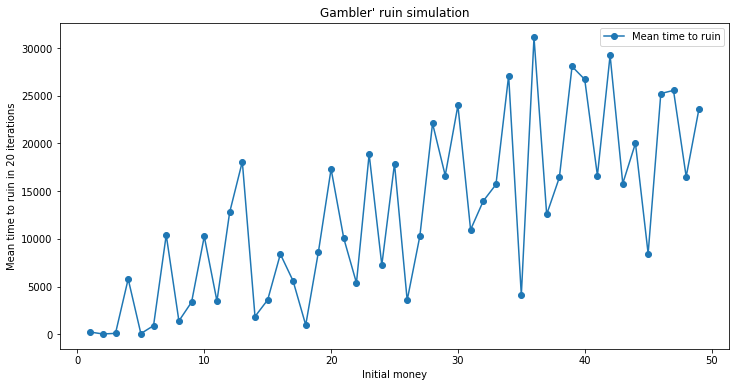
\includegraphics[scale=.6]{figures/gambler1}
	\centering
	\caption{Mean time of 50 simulations of Gambler's Ruin process}
\end{figure}

\textbf{Apartado b)} Estimar media y varianza (usar unas 20 ejecuciones, deberían ser más que suficientes) considerando un dinero inicial de $\{1, \ldots, 50\}$ euros. Indicar media y varianza. ¿Cómo varían la media y la varianza cuando aumenta el dinero inicial? \\

Para este segundo apartado repetimos el experimento anterior calculando también la desviación típica sobre esas 20 repeticiones. Puesto que queremos visualizar cómo afecta la varianza de las ejecuciones a la salida del modelo, representaremos en el gráfica también la desviación típica. Adicionalmente, como estimación más realista de la dispersión de las medidas podemos utilizar un intervalo de confianza. En particular, hemos utilizado intervalos de confianza que asumen que las mediciones se distribuyen según una distribución normal, lo que no tendría por qué ser exactamente cierto. La fórmula utilizada para dichos intervalos es la siguiente:

\[
	\text{IC} = [ \bar x - \frac{\sigma \cdot z}{\sqrt n}, \bar x + \frac{\sigma \cdot z}{\sqrt n}  ]
\]

Donde para nivel de significación $\alpha = 0.05$, $z_{1 - 0.05/2} = z_{0.975}$ es el percentil $0.975$ de la distribución normal. Veámos los resultados obtenidos:

\begin{minted}{python}
def mean_and_std_of_ruin_time(initial_money, n=20, max_steps=10**5, p=1/2):
	times = [simulate_gamblers_ruin(initial_money, p=p, max_steps=max_steps)
	for _ in range(n) ]
	return np.mean(times), np.std(times)

def compute_clipped_CI(mean, std, n, alpha=0.05):
	z = stats.norm.ppf(1 - alpha/2)
	std_error = abs(std * z / np.sqrt(n))
	return max(mean - std_error, 0), mean + std_error

def plot_ruin_time_estimation(max_initial_money=50, n=20, max_steps=10**5, p=1/2):
	"""
		Plots the mean time for a gambler's to ruin themself, against the initial money.
		- max_initial_money: max initial money to be plotted
		- n: the number of 
		- p: the probability of winning at each step
	"""
	# Compute times
	initial_money_range = np.arange(1, max_initial_money)
	mean_and_stds = np.array([mean_and_std_of_ruin_time(initial_money, n=n, max_steps=max_steps, p=p)
								for initial_money in initial_money_range])
	intervals = np.array([ compute_clipped_CI(mean, std, n) for mean, std in mean_and_stds])
	CI_std_min, CI_std_max = np.max(mean_and_stds[:,0] - mean_and_stds[:,1], 0), mean_and_stds[:,0] + mean_and_stds[:,1]
	
	# Plotting
	plt.figure(figsize=(12,6))
	plt.plot(initial_money_range, mean_and_stds[:,0], '-o')
	plt.fill_between(initial_money_range, CI_std_min, CI_std_max, color='green', alpha=.3)
	plt.fill_between(initial_money_range, intervals[:,0], intervals[:,1], color='b', alpha=.3)
	plt.legend(['Mean time to ruin', '+- Std', 'Confidence interval'])
	plt.xlabel('Initial money')
	plt.ylabel('Mean time to ruin in {} iterations'.format(n))
	plt.title('Gambler\' ruin simulation')
	plt.show()
	
random.seed(123)
plot_ruin_time_estimation()
\end{minted}

\begin{figure}[H]
	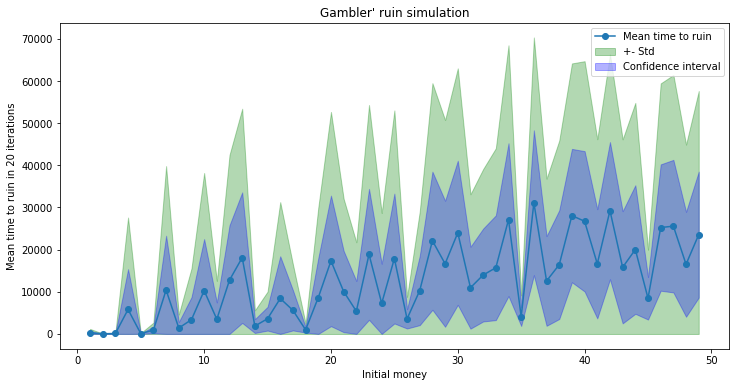
\includegraphics[scale=.6]{figures/gambler2}
	\centering
	\caption{Mean, std and normal confidence interval for the ruining time, 20 executions.}
\end{figure}

Vemos en la figura anterior como tanto el intervalo de confianza como la deviación típica aumentan gradualmente al incrementar el dinero inicial. Algunas de estas simulaciones acababan llegando al límite de $10^5$ impuesto. \\

Vemos también como hay mucha fluctuación para los valores medios. Por ejemplo, apreciamos cierto punto entre $30$ y $40$ euros iniciales que toma valores bajísimos en todas sus ejecuciones (por esto la desviación típica es también tan pequeña). Esto nos indica que quizás $20$ ejecuciones para esta simulación no nos dan una estimación correcta de la media y varianza. Volvemos a lanzar el experimento para $100$ ejecuciones y obtenemos los siguientes resultados:

\begin{minted}{python}
random.seed(123)
plot_ruin_time_estimation(n=100)
\end{minted}

\begin{figure}[H]
	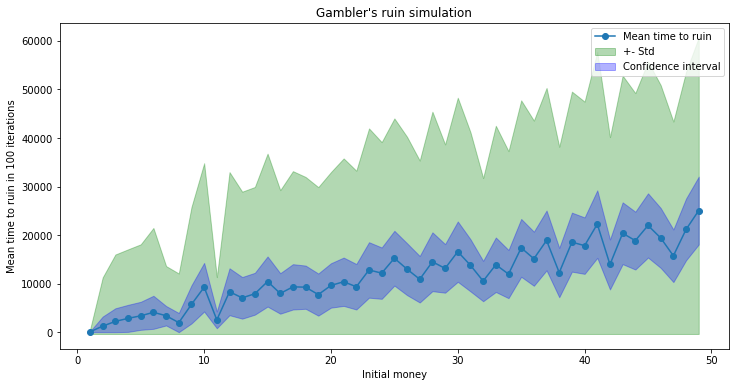
\includegraphics[scale=.6]{figures/gambler2_1}
	\centering
	\caption{Mean, std and normal confidence interval for the ruining time, 100 executions.}
\end{figure}

Podemos apreciar que se reduce enormemente la comentada variabilidad: los valores obtenidos están mucho más alineados no hay tanta oscilación. Sin embargo, han aumentado tremendamente los valores medios entre este experimento y el anterior. Este se debe a que muchas más simulaciones han alcanzado el límite de tiempo impuesto, y la media sube enormemente. A pesar de ello, \textbf{podemos deducir que tanto el número de simulaciones que alcanzan el límite como el tiempo media crecen de forma lineal}. Este resultado será clave para el próximo apartado. \\

Por otro lado, es claro que al imponer este límite en las iteraciones estamos introduciendo un sesgo en los resultados: el tiempo medio aumenta considerablemente. Sin embargo, imponer un límite más alto sólo introduce un mayor sesgo. La conclusión es clara: \textbf{es realmente complicado obtener estimaciones insesgadas y precisas del tiempo que tarda el jugador en arruinarse}, debido al elevadísimo tiempo que medio que conlleva.

\textbf{Apartado c)} Dar una estimación de la función $T(e)$ que da el tiempo medio necesario para arruinarse en función de la cantidad inicial de dinero, e. Según esta función, ¿cuánto tarda el jugador en arruinarse si empieza a jugar con 200 Euros? \\

Por el resultado expuesto en el apartado anterior, sabemos que una estimación lineal será adecuada. Es por ello que utilizaremos regresión lineal. Sin embargo, como también ha sido previamente comentado, cuantas más ejecuciones realizamos mayor será el sesgo introducido. Por otro lado, para pocas iteraciones, la varianza es muy alta y tendremos un mayor error. Realizaremos pues dos estimaciones: para $20$ y $100$ ejecuciones respetivamente.

\begin{minted}{python}
def plot_ruin_time_regression(max_initial_money=50, n=20, max_steps=10**5, p=1/2, display_prediction=True):
	"""
	Plots the mean time for a gambler's to ruin themself, against the initial money.
	- max_initial_money: max initial money to be plotted
	- n: the number of 
	- p: the probability of winning at each step
	"""
	# Compute times
	initial_money_range = np.arange(1, max_initial_money)
	mean_and_stds = np.array([mean_and_std_of_ruin_time(initial_money, n=n, max_steps=max_steps, p=p)
								for initial_money in initial_money_range])
	intervals = np.array([ compute_clipped_CI(mean, std, n) for mean, std in mean_and_stds])
	CI_std_min, CI_std_max = np.max(mean_and_stds[:,0] - mean_and_stds[:,1], 0), mean_and_stds[:,0] + mean_and_stds[:,1]

	# Compute regression
	X = initial_money_range.reshape(-1, 1)
	y = mean_and_stds[:,0].reshape(-1, 1)
	reg_model = LinearRegression().fit(X, y)
	predictions = reg_model.predict(X)
	
	# Display the prediction for 200 initial money
	if display_prediction:
		result = reg_model.predict(np.array([[200]]))
		print('Prediction for 200 initial money (n={}): {}'.format(n, result[0,0]))

	# Plotting
	plt.figure(figsize=(12,6))
	plt.plot(initial_money_range, mean_and_stds[:,0], '-o')
	plt.plot(initial_money_range, predictions, color='r')
	plt.fill_between(initial_money_range, CI_std_min, CI_std_max, color='green', alpha=.3)
	plt.fill_between(initial_money_range, intervals[:,0], intervals[:,1], color='b', alpha=.3)
	plt.legend(['Mean time to ruin', 'linear regression', '+- Std', 'Confidence interval'])
	plt.xlabel('Initial money')
	plt.ylabel('Mean time to ruin in {} iterations'.format(n))
	plt.title('Gambler\'s ruin simulation')
	plt.show()
	
random.seed(123)
plot_ruin_time_regression()
\end{minted}

\begin{minted}{bash}
	Prediction for 200 initial money (n=20): 94067.22283163268
\end{minted}

\begin{figure}[H]
	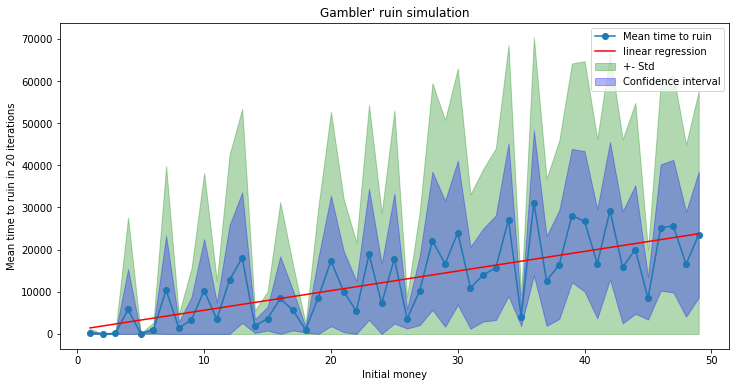
\includegraphics[scale=.6]{figures/gambler3}
	\centering
	\caption{Lineal regression for the ruining time, 100 executions.}
\end{figure}


\begin{minted}{python}
random.seed(123)
plot_ruin_time_regression(n=100)
\end{minted}

\begin{minted}{bash}
	Prediction for 200 initial money (n=100): 83077.38566326529
\end{minted}

\begin{figure}[H]
	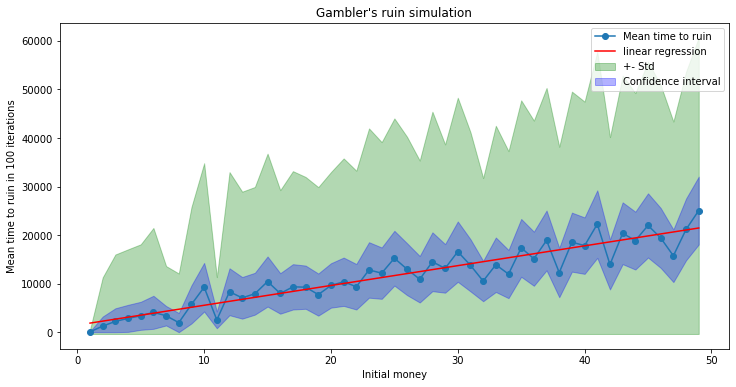
\includegraphics[scale=.6]{figures/gambler3_1}
	\centering
	\caption{Lineal regression for the ruining time, 100 executions.}
\end{figure}

Obtenemos así dos predicciones, entre las cuales la más cercana al valor real -sesgado por el límite introducido- será la segunda: $83077.39$ será el tiempo medio que el jugador tardará en arruinarse. Suponiendo que una iteración del juego tarde $1$ minuto, el jugador tardaría en arruinarse, de media, $57.69$ días (sin parar de jugar).


\section*{Ejercicio III.}

\textbf{Enunciado.} En los apuntes hay el ejemplo del \emph{gambler's ruin} como cadena de Markov:


\end{document}
